\documentclass{article}

\usepackage{fancyhdr}
\usepackage{extramarks}
\usepackage{amsmath}
\usepackage{amsthm}
\usepackage{amsfonts}
\usepackage{tikz}
\usepackage[plain]{algorithm}
\usepackage{algpseudocode}
\usepackage[encapsulated]{CJK}
\usepackage{graphicx}
\usepackage{caption}
\usepackage{subcaption}
\usepackage{graphics, tikz, tkz-berge, tkz-graph}
\graphicspath{ {./images/} }

\usetikzlibrary{automata,positioning}

%
% Basic Document Settings
%

\topmargin=-0.45in
\evensidemargin=0in
\oddsidemargin=0in
\textwidth=6.5in
\textheight=9.0in
\headsep=0.25in

\linespread{1.1}

\pagestyle{fancy}
\lhead{\hmwkAuthorName}
\chead{\hmwkClass\:\hmwkTitle}
\rhead{\firstxmark}
\lfoot{\lastxmark}
\cfoot{\thepage}

\renewcommand\headrulewidth{0.4pt}
\renewcommand\footrulewidth{0.4pt}

\setlength\parindent{0pt}

%
% Create Problem Sections
%

\newcommand{\enterProblemHeader}[1]{
    \nobreak\extramarks{}{Problem \arabic{#1} continued on next page\ldots}\nobreak{}
    \nobreak\extramarks{Problem \arabic{#1} (continued)}{Problem \arabic{#1} continued on next page\ldots}\nobreak{}
}

\newcommand{\exitProblemHeader}[1]{
    \nobreak\extramarks{Problem \arabic{#1} (continued)}{Problem \arabic{#1} continued on next page\ldots}\nobreak{}
    \stepcounter{#1}
    \nobreak\extramarks{Problem \arabic{#1}}{}\nobreak{}
}

\setcounter{secnumdepth}{0}
\newcounter{partCounter}
\newcounter{homeworkProblemCounter}
\setcounter{homeworkProblemCounter}{1}
\nobreak\extramarks{Problem \arabic{homeworkProblemCounter}}{}\nobreak{}

%
% Homework Problem Environment
%
% This environment takes an optional argument. When given, it will adjust the
% problem counter. This is useful for when the problems given for your
% assignment aren't sequential. See the last 3 problems of this template for an
% example.
%
\newenvironment{homeworkProblem}[1][-1]{
    \ifnum#1>0
        \setcounter{homeworkProblemCounter}{#1}
    \fi
    \section{Problem \arabic{homeworkProblemCounter}}
    \setcounter{partCounter}{1}
    \enterProblemHeader{homeworkProblemCounter}
}{
    \exitProblemHeader{homeworkProblemCounter}
}

%
% Homework Details
%   - Title
%   - Due date
%   - Class
%   - Section/Time
%   - Instructor
%   - Author
%

\newcommand{\hmwkTitle}{Homework\ \#14}
%\newcommand{\hmwkDueDate}{September 17, 2015}
\newcommand{\hmwkClass}{Graph Theory}
\newcommand{\hmwkClassTime}{}
\newcommand{\hmwkClassInstructor}{}
\newcommand{\hmwkAuthorName}{Lin Hung Cheng B01902059}

%
% Title Page


\title{
    \vspace{2in}
    \textmd{\textbf{\hmwkClass:\ \hmwkTitle}}\\
    %\normalsize\vspace{0.1in}\small{Due\ on\ \hmwkDueDate\ at 3:10pm}\\
    %\vspace{0.1in}\large{\textit{\hmwkClassInstructor\ \hmwkClassTime}}
    \vspace{3in}
}

\author{\textbf{\hmwkAuthorName}}
\date{}

\renewcommand{\part}[1]{\textbf{\large Part \Alph{partCounter}}\stepcounter{partCounter}\\}

%
% Various Helper Commands
%

% Useful for algorithms
\newcommand{\alg}[1]{\textsc{\bfseries \footnotesize #1}}

% For derivatives
\newcommand{\deriv}[1]{\frac{\mathrm{d}}{\mathrm{d}x} (#1)}

% For partial derivatives
\newcommand{\pderiv}[2]{\frac{\partial}{\partial #1} (#2)}

% Integral dx
\newcommand{\dx}{\mathrm{d}x}

% Alias for the Solution section header
\newcommand{\solution}{\textbf{\large Solution}}

% Probability commands: Expectation, Variance, Covariance, Bias
\newcommand{\E}{\mathrm{E}}
\newcommand{\Var}{\mathrm{Var}}
\newcommand{\Cov}{\mathrm{Cov}}
\newcommand{\Bias}{\mathrm{Bias}}

\begin{document}

\maketitle

\pagebreak



\begin{homeworkProblem}
  \begin{CJK}{UTF8}{bsmi} % 開始 CJK2

    \textbf{1.}

    設在最多12點的平面圖中,存在著色數為5的圖(五色定理)。\\
令G為著色數5的圖中最小的圖,移除其度數不大於4的點v,此時的圖$G'$著色數為4,否則G不為著色數5的圖中最小的圖。\\
    重新加入此點,可發現其著色數為4,矛盾:\\
    若其度數小於4,v可填原本的4色之一,著色數為4。\\
    若其度數等於4且其鄰居有兩個以上同色,v可填原本的4色之一,著色數為4。\\
    若其度數等於4且其鄰居分別用4種不同色,則使用5色定理證明時的方法換色即可。\\

    \proof
    最多12點的平面圖中, 除了正二十面體,存在度數不大於4的點。\\
    最多12點的平面圖邊數最多為30,此時若要建構出所有點度數大於4,則每個點度數均為5,即為正二十面體。\\

    所以上述證明了除了正二十面體,設在最多12點的平面圖中,存在著色數為5的圖(五色定理)。\\

    正二十面體的著色如下:

    \begin{figure}[h]
      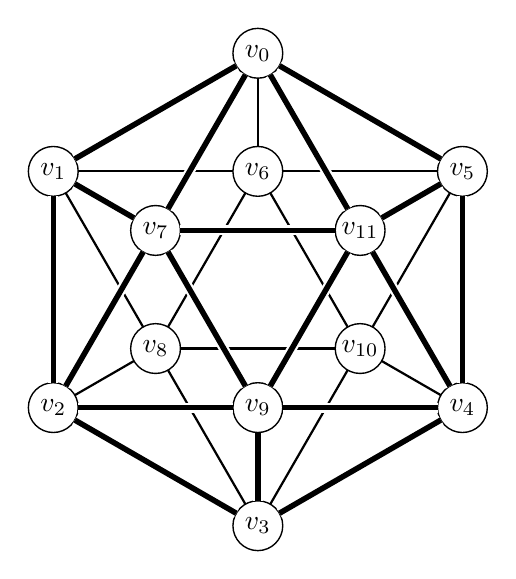
\begin{tikzpicture}
        \begin{scope}[rotate=90]
          \SetVertexNoLabel   % <--- This avoids that default $a_0$, .. $b_0$ labels show up
          \grIcosahedral[form=1,RA=3,RB=1.5]

          % Following two lines assign labels to a-like and b-like nodes
          % change it as you prefer
          \AssignVertexLabel{a}{$v_0$, $v_1$, $v_2$, $v_3$, $v_4$, $v_5$};
          \AssignVertexLabel{b}{$v_6$, $v_7$, $v_8$, $v_9$, $v_{10}$, $v_{11}$};

          % The remaining code is unchanged
          \SetUpEdge[color=white,style={double=black,double distance=2pt}]
          \EdgeInGraphLoop{a}{6}
          \EdgeFromOneToSel{a}{b}{0}{1,5}
          \Edges(a2,b1,b3,b5,a4)
          \Edge(a3)(b3)
          \Edges(a1,b1,b5,a5)
          \Edges(a2,b3,a4)
        \end{scope}
      \end{tikzpicture}
    \end{figure}
    
    \textbf{2.}

    在最多32條邊的圖中,若點數最多為12,已證明。\\
    若點數$\geq$13,則其平均度數$<5$,必存在度數小於四的點,\\
    用相同方法即可證明。
    
\end{CJK} % 結束 CJK 環境 
\end{homeworkProblem}

\pagebreak

\begin{homeworkProblem}
  \begin{CJK}{UTF8}{bsmi} % 開始 CJK3
    \solution
    
    考慮$G_2$的情形,由列舉可知$G_2$的4著色會使4色均使用2次。設$G_n$成立,則$G_{n+2}$即為$G_n$的外圈四點及$G_2$的內圈四點分別相連的圖形。此時$G_n$使4色均使用n次;而$G_2$的部份,可用以下規則連接$G_n$和$G_2$,使$G_{n+2}$的4著色使4色均使用n+2次,由數學歸納法得證。\\
    $G_n$的外圈四點為$P_1$ 到 $P_4$,有邊$\{$$P_1$, $P_2$$\}$, $\{$$P_2$, $P_3$$\}$, $\{$$P_3$, $P_4$$\}$, $\{$$P_4$, $P_1$$\}$\\
    $G_2$的八個點為$p_1$ 到 $p_8$,有邊$\{$$p_1$, $p_2$$\}$, $\{$$p_2$, $p_3$$\}$, $\{$$p_3$, $p_4$$\}$, $\{$$p_4$, $p_1$$\}$, $\{$$p_5$, $p_6$$\}$, $\{$$p_6$, $p_7$$\}$, $\{$$p_7$, $p_8$$\}$, $\{$$p_8$, $p_5$$\}$, $\{$$p_1$, $p_5$$\}$, $\{$$p_2$, $p_5$$\}$, $\{$$p_2$, $p_6$$\}$, $\{$$p_3$, $p_6$$\}$, $\{$$p_3$, $p_7$$\}$, $\{$$p_4$, $p_7$$\}$, $\{$$p_4$, $p_8$$\}$, $\{$$p_1$, $p_8$$\}$。\\
    相連的邊為$\{$$P_1$, $p_1$$\}$, $\{$$P_2$, $p_1$$\}$, $\{$$P_2$, $p_2$$\}$, $\{$$P_3$, $p_2$$\}$, $\{$$P_3$, $p_3$$\}$, $\{$$P_4$, $p_3$$\}$, $\{$$P_4$, $p_4$$\}$, $\{$$P_1$, $p_4$$\}$\\
    (1) 若$G_n$的外圈四點著色組合為$\{$x, x, y, y$\}$,不失一般性,令$P_1$ 到 $P_4$ 為$\{$x, y, x, y$\}$,\\
    則$p_1$到$p_8$可著色為$\{$w, z, w, z, x, y, x, y$\}$\\
    (2) 若$G_n$的外圈四點著色組合為$\{$x, x, y, z$\}$,不失一般性,令$P_1$ 到 $P_4$ 為$\{$x, y, x, z$\}$, \\
    則$p_1$到$p_8$可著色為$\{$z, w, z, y, x, y, x, w$\}$\\
    (3) 若$G_n$的外圈四點著色組合為$\{$w, x, y, z$\}$,不失一般性,令$P_1$ 到 $P_4$ 為$\{$w, x, y, z$\}$,\\
    則$p_1$到$p_8$可著色為$\{$y, z, w, x, z, w, y, z$\}$\\
    
  \end{CJK} % 結束 CJK 環境 
\end{homeworkProblem}

\begin{homeworkProblem}
  \begin{CJK}{UTF8}{bsmi} % 開始 CJK4

    \solution

    \textbf{1. }

    在圖的外圍加上一個點v,並將所有點連至此點。因為是外圍平面圖,新的圖G必為平面圖。\\
    此時G可被4著色。因為v連至所有點,v的顏色不能用於原圖中的任一點。所以原圖可被3著色。

    \textbf{2.}

    1個點的外圍平面圖可被3著色。\\
    設n個點的外圍平面圖可被3著色,則在$G_{n+1}$中取一度數不大於2的點v,移除v和其邊。此時圖為n個點的外圍平面圖。\\
    可以將v著色為與其鄰居皆不同的顏色,此時最多只用3色,所以$G_{n+1}$可被3著色;由數學歸納法得證。

    \textbf{3.}
    將圖分割成互不相交的三角形,其頂點均為原圖的點。此時的圖G為外圍平面圖,將圖G著色成3色,且因為三角形的三個點顏色兩兩不同,所以選擇最少出現的顏色作為守衛的位置即得證。
    
  \end{CJK} % 結束 CJK 環境    
\end{homeworkProblem}

\begin{homeworkProblem}
  \begin{CJK}{UTF8}{bsmi} % 開始 CJK5

    \solution

    在環上,對一個至少有三個點的圖,永遠有e $\leq$ 3n。\\
    \proof 
    環面的虧格為1,所以$n-e+f=0$。\\
    且因為n$\geq$3,且於環面上,每個面都至少有三條邊。\\
    $2e \geq 3f$ 代入公式後就得到 $e \leq 3n$。\\

    將圖分割成互不相交的三角形,其頂點均為原圖的點。此時每個面都由三條邊組成,所以$2e = 3f$,$e = 3v$,且每點度數均為6。\\
    所以在環上,一個至少有三個點的圖的著色數$\leq$7,且因為$K_7$可以嵌入環中,所以著色數$\geq$7。

  \end{CJK} % 結束 CJK 環境    
\end{homeworkProblem}

\end{document}

%%% Local Variables:
%%% mode: latex
%%% TeX-master: t
%%% End:
